%%%%
\chapter{まとめと課題} \label{conclusion}

\section{まとめ}
本研究では、学習者に物理系を定義させるシミュレータである \simname~(\simnamealt) を提案した。\simname では、物理法則から現象を数式で記述し、シミュレーションに変換するまでの工程も学習者が行う。これにより、従来は授業などで教わる必要があった現実の物理現象と物理法則の間の対応を学習者自らの経験を通して理解することができる。

\section{今後の課題}

\subsection{実装}

現在 \simname の機能のうち、
\begin{enumerate}
  \item 学習者の入力を Equation として解釈する
  \item 不正な次元の方程式になっていないかを確認する
  \item 数値計算するために数値を与える必要のある変数を推論する
\end{enumerate}
という部分が未実装である。それぞれについて方針を述べる。

\subsubsection*{学習者の入力を Equation として解釈する}
入力の解釈は、sympy.parsing.sympy\_parser の parse\_expr 関数を使うことで可能である。この関数では、文字列を SymPy のSymbol, Sum, Mul や Eq などに変換できる。実際に行う例を図~\ref{example_parse}に示す。一方、単にこれを用いるだけでは未定義の変数を使うことができてしまう。そのため、解釈された変数が定義されたものなのかを確認する必要がある。また、学習者がアンダースコアなどを入力する必要があったり、意図しない解釈をされる($v_Ax$ と $v_{Ax}$ など)可能性がある。Jupyter に表示されている変数をクリックすることでその変数を入力することができれば、このような誤りは防止でき、学習者の入力にかかる手間も減らすことができる。

\begin{figure}[htb]
  \centering
  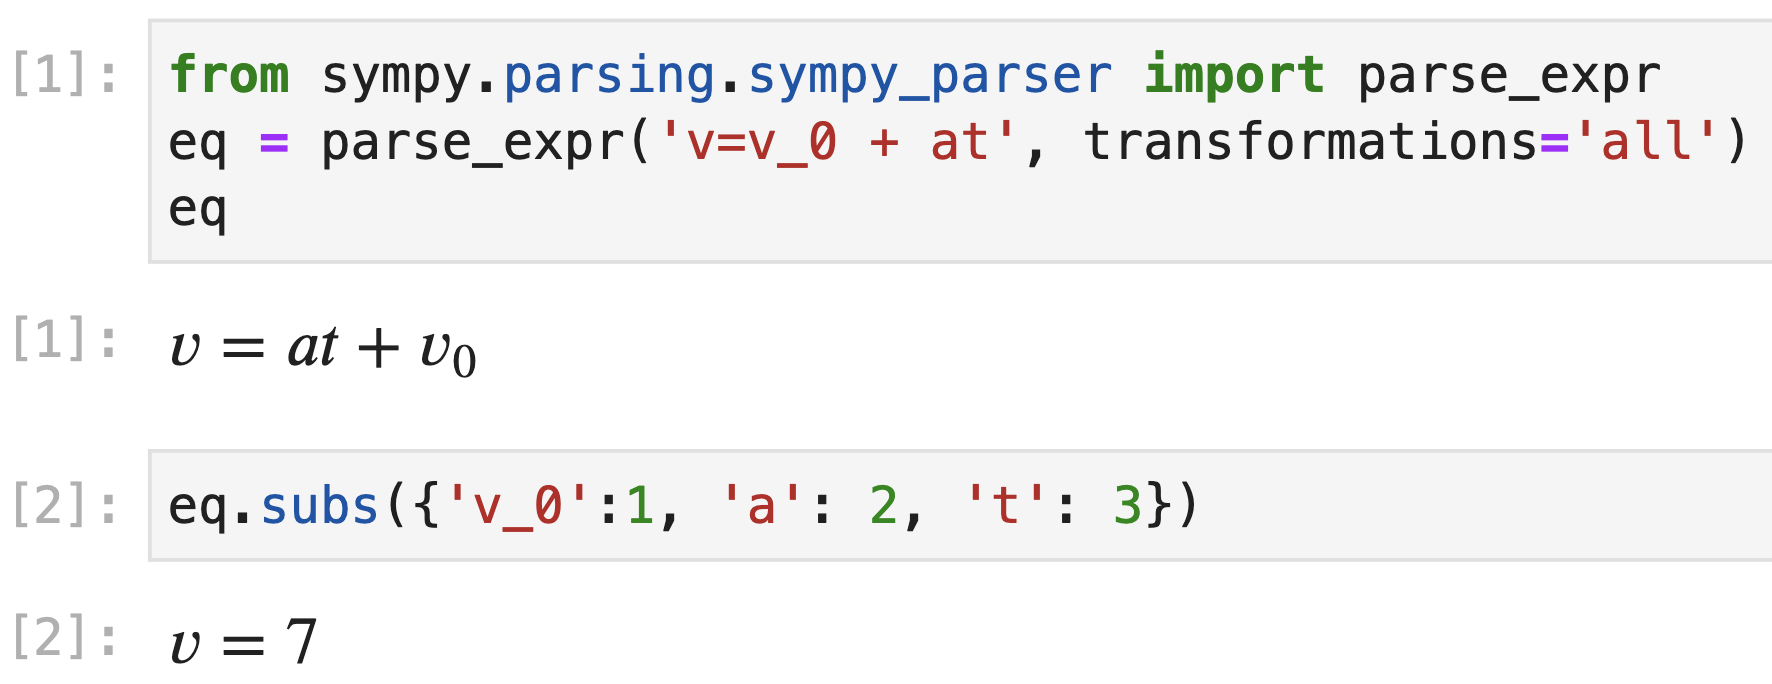
\includegraphics[width=0.9\linewidth]{work/example_parse.png}
  \caption{parse\_expr 関数で文字列をパースする例} \label{example_parse}
\end{figure}

\subsubsection*{不正な次元の方程式になっていないかを確認する}
現在の実装では、 $g + t~~\mathrm{([L/T^2] + [T])}$ のように次元が不正な方程式も定義できてしまう。SymPy の変数に次元の情報を付加し、異なる次元間の加減などを検出する必要がある。自動で追加される変数は生成する際に次元の情報を付加すればよいが、学習者が新たに追加する変数については次元を手動で指定する必要がある。L, M, T などの組み合わせを文字列で入力したものを解釈する、各次元の指数を数値で入力したものを解釈するなどの方法が考えられる。

\subsubsection*{数値計算するために数値を与える必要のある変数を推論する}
基本的には、学習者が定義した方程式に含まれる変数のうち物体に紐づいている位置・速度以外の変数の値を入力させれば良い。しかし、次のような場合も存在する。
\begin{align*}
x_A = X
X = v_0t
\end{align*}
ここで、$x_A$ は物体の $x$ 座標を表す変数で、$X$ と $v_0$ は学習者が定義した変数である。先述した方針では、$X$ と $v_0$ に値を入力する必要がある。しかし実際は $X$ か $v_0$ の一方にのみ値を入力すればよい。このような場合に対応する方法を考える必要がある。

\subsection{評価}

実装が完成したら、\simname の教育効果を評価する必要がある。高校生を、\simname を用いるグループ・PhET を用いるグループ・座学のグループに分け、pretest と posttest を行う。その結果を Hake~\cite{hake_1998}が導入した Normalized Gain を用いて比較することで、\simname の教育効果を測定できると考える。

また、\simname の利点は、現実の運動を確認できるだけでなく、現実の物理現象と物理法則の間の対応を学習者自らの経験を通して理解することができるという点である。そのため、各グループでディスカッションを行い、その内容からどれだけ現実の物理現象を正しく理解できているかを確認することも有効であると考える。

\clearpage
\section{発展のアイデア}

\simname を発展させるアイデアがいくつかあるので紹介する。

\subsection{他分野への対応}

現在の \simname の構成では、力学以外の分野に対応することが難しい。物体を追加した際の次元付き変数や観測ペインの可視化が力学を前提とした設計となっているためである。一方、高等学校で扱う物理には、音や光などの波動分野、回路や電場・磁場などの電磁気分野なども存在する。そのため、これらの分野にも対応できるようにしたい。

\subsection{方程式計算の強化}

現在、\simname 上に方程式を入力する際、その方程式の導出は学習者が行う必要がある。しかし、移項した際の符号の変え忘れや係数の間違いなど、\simname では検出できないミスが存在する。この作業を \simname でサポートしたい。

\subsubsection*{求解の自動化}
現在想定している \simname の実装では、物体に紐付けられている変数は他の変数で明示的に表されている必要がある。すなわち、$v_{Ax} = \sqrt{2gh}$ という表記は正しいが、$mgh = \dfrac{1}{2}mv_{Ax}^2$ という表記は受け付けない。このようなとき、SymPy を用いて $v_{Ax}$ を求めることができるため、計算ミスを防ぐことができる。一方、これを全て自動化してしまうと、学習者自身の方程式を変形する能力が成長しない。そのため、自動で求解するかどうかを切り替えられるようにする必要がある。

\subsubsection*{基本的な公式(運動方程式、力学的エネルギー保存則等)の提供}
物理学では、頻出する公式の数はある程度限られている。基本的な公式を提供し、各値に変数を割り当てるだけ方程式を定義することができるようにすれば、学習者の負担を大きく軽減することができる。これと先述した自動求解を組み合わせることで、適切な公式を選び適切に変数を割り当てるだけで物理系が作成できる。また、公式を解説付きで一覧にしたり、公式の検索機能をつけることで、公式を覚えきれてない初学者に対してもサポートができる。
